% Chapitre 1 : Introduction
\chapter{Introduction}\label{chapter:01:introduction}
{
    \section{Diagnostics du cancer de la prostate}\label{section:contexte} % "par coupes histologies" en plus ?
    {
        \emph{Ce stage, financé par le LabEx NUMEV, s'inscrit dans le cadre d'une collaboration internationale entre l'université de Tulane dans la ville de Nouvelle Orléans, et l'université de Montpellier sur un projet d'aide à la détection du cancer de la prostate.}\medskip

        Le cancer de la prostate est aujourd'hui diagnostiqué grâce à l'échelle de Gleason (décrite à la section \ref{section:gleason_scale}) qui représente les contours des glandes de la prostate à différent stade de la maladie. L'échelle de Gleason est construite à partir de coupes histologiques\definition{Coupes effectuées dans un tissu biologique} planaires et comporte des croquis de chaque type de glandes. Cette méthode de diagnostic présente une grande variabilité selon l'opérateur (figure \ref{img:gleason_bias}). Ces différences dans le diagnostic peuvent être expliquées par deux facteurs: la variance de la forme des glandes engendrée par le choix de l'orientation des plans de coupe dans le tissu, mais aussi par le manque de précision des dessins servant de référence dans l'échelle de Gleason (figure \ref{img:gleason_scale}). Afin d'améliorer le diagnostic du cancer de la prostate, il apparaît nécessaire de développer de nouvelles techniques de détection de structures cancéreuses. L'approche envisagée ici est l'étude tridimensionnelle de la forme des glandes dans un échantillon de prostate, permettant ainsi d'éliminer la variabilité due à l'angle de coupe dans la méthode de Gleason. Nos collaborateurs de l'université de Tulane à la Nouvelle Orléans ont pour cela développé un microscope à feuillet de lumière permettant de capturer une image 3D d'un échantillon de tissu humain (voir la section \ref{section:microscopy}). Une reconstruction volumique d'un échantillon de prostate permettra une étude morphologique et topologique des glandes afin d'enrichir les méthodes de diagnostic du cancer.

        \begin{figure}[h]
            \centering
            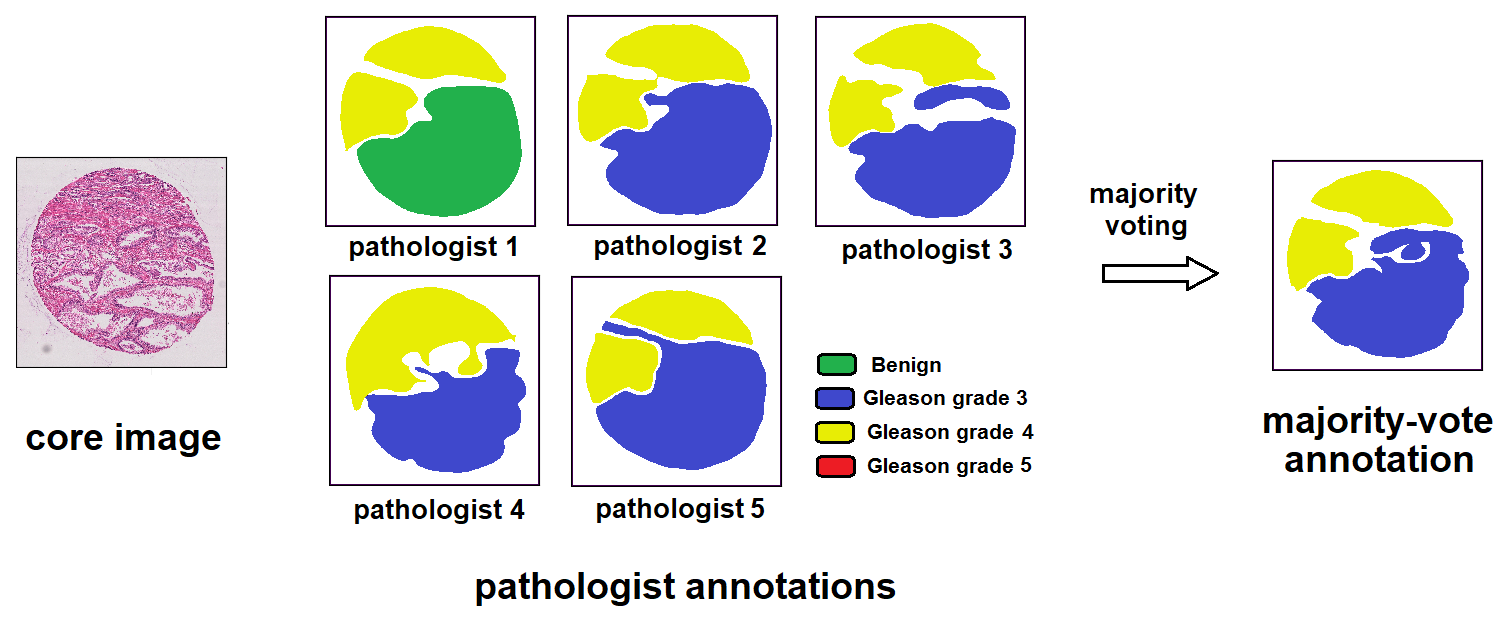
\includegraphics[width=.7\linewidth]{img/gleason_bias.png}
            \captionsetup{width=.8\linewidth, labelfont=bf}
            \caption{Variabilité inter-opérateur pour les diagnostics de l'échelle de Gleason d'un même échantillon.\cite{cite_gleason_bias}}
            \label{img:gleason_bias}
        \end{figure}
        
        Le microscope créé par les chercheurs de l'université de Tulane est extrêmement précis, générant des images dont la résolution spatiale est inférieure au micromètre. Leur technique d'acquisition (voir section \ref{section:microscopy} pour plus d'informations) nécessite l'utilisation de deux capteurs en tandem effectuant des vues par coupe de l'échantillon. Cela génère, pour une seule acquisition, deux piles d'images correspondant à des points de vue différents. Ces deux piles d'images doivent donc être fusionnées de manière cohérente pour reconstruire la structure 3D et visualiser l'échantillon. Mais la taille des images, ainsi le nombre de prises de vues, rend impossible le stockage en mémoire vive d'une acquisition. Cela rend l'analyse de l'échantillon particulièrement complexe.
        }
        
\section{Objectif du stage: Vers une modélisation 3D des glandes de la prostate}\label{section:contrib}
    {
        L'objectif de ce stage est de proposer un système de visualisation interactive des données, permettant une première exploration de la forme des glandes. Notre travail comporte deux axes principaux. Le premier axe présente plusieurs méthodes de visualisation permettant d'afficher un jeu de données massif: une exploration par plans de coupes ou une visualisation volumique par sous-domaine. %Afin d'atteindre cet objectif, une prise en main des outils de développement sera nécessaire, pour se familiariser avec les jeux de données. Ensuite, il nous faudra établir une méthode permettant la gestion des données, afin de pouvoir les afficher à l'écran, et les manipuler en temps réel.
        Les données ne pouvant pas rentrer en mémoire sur des stations de travail standard, une première méthode de pré-traitement pour la visualisation sera mise en place, ne chargeant qu'une version basse résolution des images. Pour finir, nous proposerons deux méthodes de visualisations pour les jeux de données. Une première méthode permettra une exploration interactive des jeux de données chargés en mémoire par l'utilisation de plans de coupe. Ensuite, une autre méthode de visualisation par sous-domaine sera présentée. Cette méthode fut originellement développée pour visualiser des images segmentées, mais peut être adaptée pour visualiser des images non-segmentées. Les travaux réalisés sur la méthode de visualisation par sous-domaines ont fait l'objet d'une soumission à la conférence IEEE VIS 2020, en collaboration avec Mme \textsc{Faraj} ainsi que M.\textsc{Summa}.

        Par la suite, il nous faudra proposer une méthode reconstruisant les deux piles présentes dans le jeu de données en une seule image médicale, en tenant compte des différentes caractéristiques des prises de vues. Pour ce faire, il faudra proposer une méthode de reconstruction prenant en compte les conditions de prises de vues particulières des piles d'images stockées en mémoire. Nous commencerons par proposer une méthode de recherche de voisins en espace affine, et continuerons sur une méthode de génération de grille prenant en compte cette recherche de voisins, afin de créer des grilles de résolution et de taille arbitraire. Afin de réduire l'empreinte mémoire, ces deux méthodes sont réalisées à la volée pour permettre le traitement d'une plus grande quantité de données.

        \iffalse
        \noindent\commentaire{Nouveau plan suggéré (majoritairement réorganisation, pas de contenu en +) :\begin{itemize}
            \item Intro
            \item partie 'prise en main' :\begin{itemize}
                \item chargement des données\begin{itemize}
                    \item présentation méthode de stockage mémoire (section 2.1 maintenant)
                    \item présentation interpolation
                \end{itemize}
                \item visu par plans de coupe (même texte)
                \item visu par sous-domaines (même texte)
            \end{itemize}
            \item partie travail de stage :\begin{itemize}
                \item présentation du problème (présentation des différents espaces depuis fig 4.1 principalement, plus présentation dual-visu en adéquation avec le problème)
                \item recherche de voisins\begin{itemize}
                    \item méthodes d'interpolation (comparaison, à faire après résultats)
                    \item implémentation
                    \item résultats (ici, ou plutot dans résultats génération grille ?)
                \end{itemize}
                \item reconstruction de grilles\begin{itemize}
                    \item méthode utilisée
                    \item implémentation
                    \item tests
                    \item résultats (à venir)
                \end{itemize}
            \end{itemize}
            \item conclusion
        \end{itemize}}
        \fi
    }
    
        
	% }}}

}
% VIM modeline : do not touch !
% vim: set spell spelllang=fr :
